\documentclass{jib}
\newlength{\platz}
\setlength{\platz}{15pt}
\RequirePackage{listings}

%\usepackage{changepage} %test, TODO remove

\lstset{%
  basicstyle=\ttfamily,
  fontadjust,
  flexiblecolumns=true,
  frame=L,
  xleftmargin=15pt,
  framesep=5pt,
  emphstyle=\rmfamily\itshape}
  

\usepackage{pdfpages}

%%%%%%%%%%%%%%%%%%%%%%%%%%%%%%%%%%%%%%%%%%%%%%%%%%%%%%%%%%
% JIB Header/Footer
%%%%%%%%%%%%%%%%%%%%%%%%%%%%%%%%%%%%%%%%%%%%%%%%%%%%%%%%%%
\jibvolume{XX} % insert volume
\jibissue{X}   % insert issue
\jibpages{XXX} % insert article ID
\jibyear{XXXX} % insert year
\makeHeaderFooter{} % leave as is
%%%%%%%%%%%%%%%%%%%%%%%%%%%%%%%%%%%%%%%%%%%%%%%%%%%%%%%%%%

\begin{document}

%%%%%%%%%%%%%%%%%%%%%%%%%%%%%%%%%%%%%%%%%%%%%%%%%%%%%%%%%%
%
% Title Page
%
%%%%%%%%%%%%%%%%%%%%%%%%%%%%%%%%%%%%%%%%%%%%%%%%%%%%%%%%%%

\begin{jibtitlepage}

\jibtitle{Synthetic Biology Open Language (SBOL) \\ Version 2.3}


%We did not provide author(s) nor author footnote(s), please complete as applicable.
% Please make sure to use unique footnote characters for each author
\jibauthor{Curtis Madsen\iref{bu}, % editors
Angel Go\~{n}i Moreno\iref{newcastle},
Umesh P\iref{kerala},
Zachary Palchick\iref{zymergen},
Nicholas Roehner\iref{bbn}, 
% 
Christian Atallah\iref{newcastle},
Bryan Bartley\iref{bbn}, 
Kiri Choi\iref{uw},
Robert Sidney Cox\iref{prospect},
Thomas Gorochowski\iref{bristol}, 
Raik Gr\"unberg\iref{kaust},
Chris Macklin\iref{amyris},
James McLaughlin\iref{newcastle},
Tramy Nguyen\iref{utah}, 
Matthew Pocock\iref{turing}, 
Meher Samineni\iref{utah}, 
James Scott-Brown\iref{imperial},
Michael Zhang\iref{utah}, 
Zhen Zhang\iref{utahstate},
Zach Zundel\iref{utah}, 
% TODO: Add SEP authors, spec writers
% steering committee & chair
Jacob Beal\iref{bbn},
Michael Bissell\iref{amyris},  
Kevin Clancy\iref{biocoder}, 
John H. Gennari\iref{uw},
Goksel Misirli\iref{keele}, 
Chris Myers\iref{utah}, 
Herbert Sauro\iref{uw},
Ernst Oberortner\iref{jgi},
Anil Wipat\iref{newcastle}\jibauthorfootnote{*}{Correspondence should be addressed to:
           \email{editors@sbolstandard.org}}}

\addjibinstitution{bu}{Boston University, USA}
\addjibinstitution{newcastle}{Newcastle University, UK}
\addjibinstitution{kerala}{Kerala Technological University, India}
\addjibinstitution{zymergen}{Zymergen, USA}
\addjibinstitution{bbn}{Raytheon BBN Technologies, USA}
\addjibinstitution{uw}{University of Washington, USA}
\addjibinstitution{prospect}{Prospect Bio, USA}
\addjibinstitution{bristol}{University of Bristol, UK}
\addjibinstitution{kaust}{KAUST, Saudi Arabia}
\addjibinstitution{amyris}{Amyris, Inc., USA}
\addjibinstitution{utah}{University of Utah, USA}
\addjibinstitution{turing}{Turing Ate My Hamster, Ltd., UK}
\addjibinstitution{imperial}{Imperial College, UK}
\addjibinstitution{utahstate}{Utah State University, USA}
\addjibinstitution{biocoder}{BioCoder Consulting, USA}
\addjibinstitution{keele}{Keele University, UK}
\addjibinstitution{jgi}{DOE Joint Genome Institute, USA}


\end{jibtitlepage}


\begin{abstract}

People who are engineering biological organisms often find it useful to communicate in
diagrams, both about the structure of the nucleic acid sequences that they are engineering 
and about the functional relationships between sequence features and other molecular species.
%
Some typical practices and conventions have begun to emerge for such
diagrams.  The Synthetic Biology Open Language Visual (SBOL Visual) has been developed as a standard 
for organizing and systematizing such
conventions in order to produce a coherent language for expressing
the structure and function 
of genetic designs. 
%
This document details version 2.1 of SBOL Visual, which builds on the prior SBOL Visual 2.0 standard by
expanding diagram syntax to include 
methods for showing modular structure and mappings between elements of a system,
interactions arrows that can split or join (with the glyph at the split or join indicating either superposition or a chemical process), 
and adding new glyphs for indicating genomic context (e.g., integration into a plasmid or genome) and for stop codons.
\end{abstract}

This document does not contain technology or technical data controlled under either the U.S. International Traffic in Arms Regulations or the U.S. Export Administration Regulations.


% Include your PDF document
%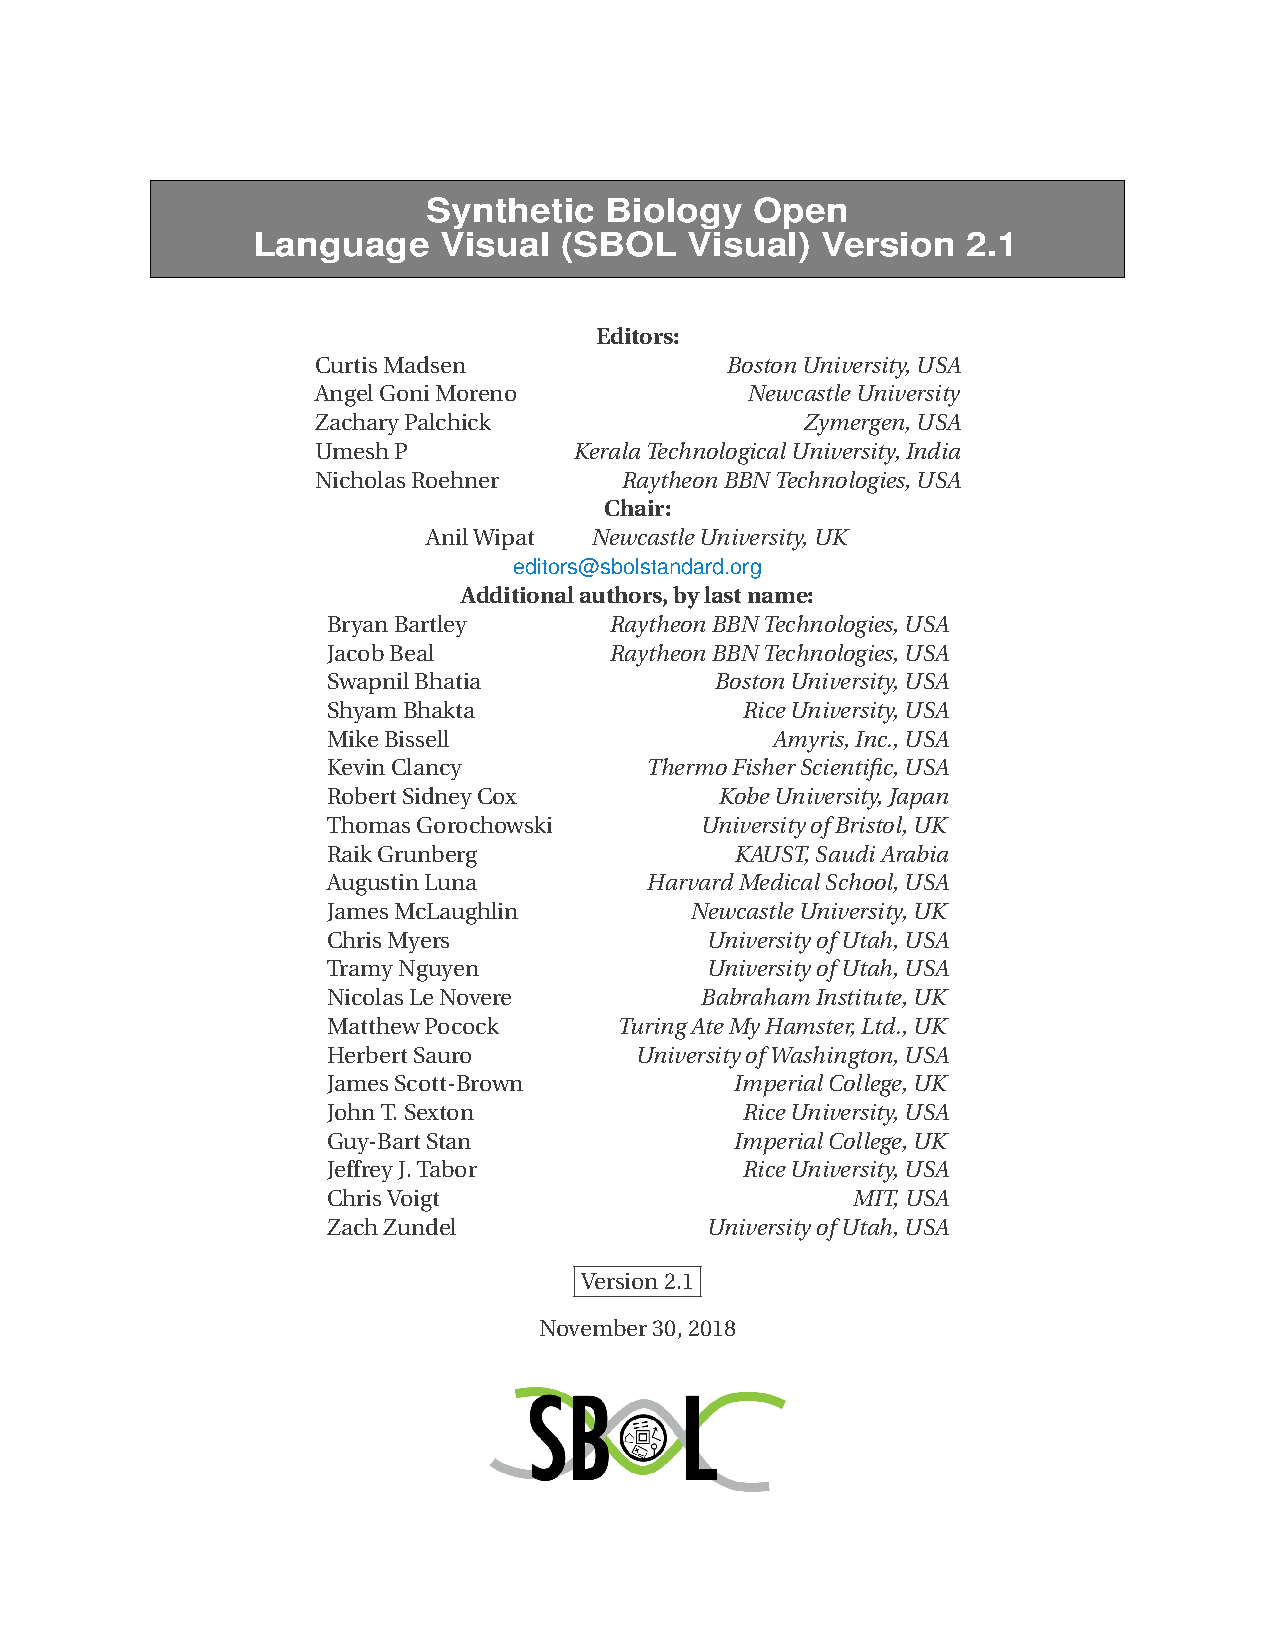
\includepdf[pages=-, offset=80 -80]{SBOL_Visual_2_1.pdf}

\end{document}
